%! Author = weiss
%! Date = 20.01.2025
\Author{\daAuthorThree}

    A well-structured backend is essential for building a scalable and maintainable application. This chapter explores the different layer of our backend. Each layer has its own purpose in handling client requests, processing logic in the code or managing database operations. Furthermore, this chapter provides an overview of the applied design principles we used in our backend.

    \begin{figure} [H]
        \centering
        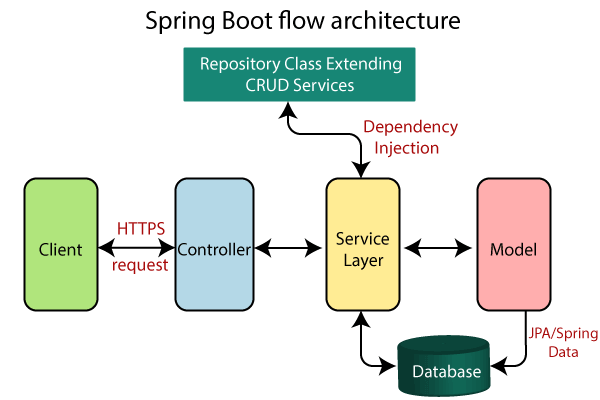
\includegraphics [width=0.75\textwidth] {images/andreas/backendstructure/springBootLayers.png}
        \caption{Layers of Spring Boot}
    \end{figure}

    \subsection{Controller Layer}
    The controller layer of a Spring Boot application is a significant layer that takes care of incoming HTTP requests and decides the appropriate response. It serves as the interface between the client and the backend which receives requests, hands over the tasks to the service layer and provides the responses accordignly. It ensures that the data which is used by the logic in the application is properly and effectively processed. \newline
    In a standard configuration, controllers handle a collection of HTTP methods. Amongst those HTTP methods are GET, POST, PUT and DELETE. Each methods has a certain function or action that are then performed by the application. Furthermore, every type of method corresponds to different operations on the data, such as retrieving, creating, updating or deleting information. Each controller belongs to a unique endpoint which serves as the interface for interacting with the application. The controller then uses service methods to execute the logic and return and appropriate response. \newline
    To ensure effective management of routing, Spring Boot uses annotations like \texttt{@GetMapping}, \texttt{@PostMapping}, \texttt{@PutMapping} and \texttt{@DeleteMapping}. These annotations identify the mapping between some of the HTTP methods and their respective handler methods in the controller. For example, the \texttt{@GetMapping} annotation is used for reading data, whereas the \texttt{@PostMapping} is applied for adding new data. The \texttt{@PutMapping} is utilized for updating existing data and the \texttt{@DeleteMapping} for deleting data. \newline
    One of the characteristics of the controller layer is the way it communicates with DTOs and entity classes. While the controller gets HTTP requests, it typically utilizes DTOs to enable data transfer between the client and the backend in a secure and effective manner.

    \subsection{Service Layer}
    The service layer plays a significant role in the backend organization to process the logic and serve as a buffer layer between the repository and controller layers. It makes the application modular, maintainable and scalable since it decouples request handling and data access. This seperation is necessary to provide flexibility in changes and additions to the application without impacting other parts of the project. \newline
    One of the primary advantages of having a dedicated service layer is that it can be reused. Rather than duplicating the logic all over the system, controllers and other code sinppets can use service methods when they need them. Not only does thi save code duplication, but it also simplifies future changes, since logic changes can be implemented in a single location without having an impact on the application overall. \newline
    Another significant aspect of this layer is transaction management. When an operation has more than one step and consists of a sequence of action, a guarantee that either all or none of those steps are executed is an absolute necessity. By defining such transactionals boundaries at the service level, the application ensures data consistency and prohibits incomplete operations from triggering undesired actions. \newline
    Wrapping complex logic within the service layer keeps the backend organized and clean. Rather than adding several conditions and operations directly into controllers or repositories, the service layer offers and organized area for processing the data. 

    \subsection{Repository Layer}
    The repository layer is in charge of managing interactions with the database by exposing efficient methods for storing, reading, updating and deleting data. By using this layer, the backend is kept modular which results in the application being more maintainable and scalable. \newline
    Spring Data JPA comes with numerous in-built methods supporting most of the common database operations. By utilizing the repository layer, operations like saving new data, getting all existing data sets, updating data and deleting data are automatically available. This cust down a lot of unnecessary code required for database operations. Furthermore, it also accelerates the development process by providing many of methods. \newline
    Although built-in repository methods cover most scenarios, there are time when more complicated queries are required. To handle such cases, Spring Data JPA supports defining custom queries through annotations. This allows developers to get certain data in an efficient way without performing unnecessary database operations.

    \subsection{Persistence Layer (Entity Classes)}
    The Spring Boot application's persistence layer handles database communication, entity classes and how different entities are related along with ensuring data consistency. With JPA in Spring Boot, developers can create a well-structured and optimized data model which enhances the performance and scalability of the application. \newline
    Entity classes are used to represent database tables and need to be defined with an annotation to be scanned by Spring Boot JPA. If the table name is different from the class name, it can be annotated explicitly. In addition, unique identifiers need to be defiend to ensure that every entity is unique.\newline
    Cascading operations automatically persistence and deletion but must be dealt with cautiously in order to not lose data. Validation maintains the integrity of data by placing contraints like mandatory fields and length limitations.\newline
    Auditing enables tracking when and by whom entities are modified which provides more accountability. Restricting field values to predefined choices guarantees information consistency and using DTOs optimize queries by retrieving only neccessary fields.

    \subsection{Applied Design Principles (DTOs)}
    During the development of a Spring Boot application, having an efficient data communication between different layers is crucial. And exactly this is where DTOs are needed. \newline
    DTOs are objects that carry data between layers in an application. They are used to encapsulate and transport data mostly between a server and a client.
    \newline
    \textbf{Why Use DTOs?} \newline
    DTOs are crucial for a backend architecture due to their abilities to enhance the security, maintainability, as well as the performance of the data. Their ability to hide data is among their major strengths because they support exposing only the necessary information to clients wihtout showing sensitive data. \newline
    From a performance-perspective, DTOs maximize network efficiency by only sending the data that is required for the current action performed by the backend. This advantage is particularly valuable in systems where bandwidth and response time are essential. \newline
    Lastly, DTOs are adaptable which allows developers to customize responses to specific use cases. They can support data combination from different entities or the exclusion of unnecessary fields which then results in more efficient responses and easier processing. \newline
    By utilizing DTOs as they are intended, applications can achieve better modulatity, security and overall performance. \newline
    \textbf{Example for Using DTOs} \newline
    A common scenatio where DTOs are useful is when managing user information in an application. \newline
    Imagine a system that stores user details such as first name, last name, email and password. If the application exposes the user data to external clients, it could lead to security risks, as sensitive information like passwords should never be shared. Instead of exposing the entire user object, a DTO can be used to filter out unnecessary or sensitive data and only transfer the relevant information. \newline
    Therefore, when a user requests a list of other users in an application, the system does not need to send private details like passwords. As an alternative, the application can create an DTO that only contains essential information, such as first name, last name and email. This would ensure that the system remains secure while still providing necessary data for the application to function properly. \newline
    DTOs also help optimizing performance by limiting the amount of data transferred. In this case, the application would send the passwords between a client and a server every time the backend needs to send data. However, by using DTOs, the application is limited by sending the first name, last name and email but not the password. \newline 
    \textbf{Best Practices for Using DTOs} \newline
    To ensure DTOs are as efficient as possible within a backend application, certain best practices should be followed. \newline 
    \textbf{Keeping DTOs Simple:}
        \begin{itemize}
            \item DTOs should only contain the necessary fields required for the specific use case that its needed for. Having too much data makes them harder to maintain and can lead to unnecessary complexity. By keeping DTOs organized, they remain efficient and can be used as they are intended.
        \end{itemize}
    \textbf{Using Validation:}
        \begin{itemize}
            \item Data validation in DTOs is required to maintain data integrity and prevent processing invalid or incomplete data. By applying validation rules, such as not allowing a field to be empty or limiting the length of different fields, errors are caught early. This prevents incorrect data from being passed on to the logic or inserted to the database.
        \end{itemize}
    \textbf{Using Automation Tools:}
        \begin{itemize}
            \item Manually constructing an DTO based off of an entity is known to create errors and to be time consuming. To simplify this, there are tools that can be used to map objects automatically. They reduce the usage of unnecessary code and speed up the development process by getting DTOs properly filled without writing manual code.
        \end{itemize}
    \textbf{Documenting the DTOs:}
        \begin{itemize}
            \item Proper documentation of every DTO created in the application is crucial. Frameworks like Swagger or SpringFox provide the possibility of auto-generated API documentation, which is easily understandable by other developers concerning the structure and expected data of each DTO. This makes collatboration easier and consistent within the project. \newline
        \end{itemize} 
    While DTOs provide numerous benefits in organizing data transfer between the layers of an application, there are some challenges that come with them. As a project grows in complexity, it may take more effort to keep the DTO approach organized. It is wise to know the possible disadvantages so that DTOs can be utilized effectively without introducing unnescessary overhead. \newline
    \textbf{Maintenance Overhead:}
    \begin{itemize}
        \item As an application evolves, the number of DTOs can grow extensively. Monitoring these DTOs, modifying them as new requirements emerge and maintaining them synchronized with the logic can prove to be an overwhelming task. Without proper structuring and an explicit DTO strategie, their maintenance can introduce excessive complexity.
    \end{itemize}
    \textbf{Performance Impact:}
    \begin{itemize}
        \item While DTOs are used to reduce the amount of data transferred over the network, mapping entities to DTOs and vice versa is extra processing. This process will be a bottleneck in performance in high-traffic applications. Using optimized mapping strategies and automated tools for this purpose can help this problem. This still needs to be taken into consideration when implementing DTOs.
    \end{itemize}
    \textbf{Consistency:}
    \begin{itemize}
        \item Keeping DTOs and entity models in sync over time is challenging. When there are any changes in the underlying data structure, it is essential that the impacted DTOs are also adjusted accordingly. If these changes are not carefully handled, inconsistencies may arise which leads to potential data mismatches and errors in API responses.
    \end{itemize}
    \textbf{Complexity:}
    \begin{itemize}
        \item In use cases involving simple data interactions, DTOs may not be required. Adding DTOs to every operation will probably add a layer of abstraction that will not be as valuable. In this scenario, working with entities directly could be a simpler and cleaner approach.
    \end{itemize}
    
